\documentclass[a4paper,10pt]{article}
\usepackage[utf8]{inputenc}
\usepackage[english]{babel}
\usepackage{graphicx}
\usepackage[nottoc]{tocbibind} %Adds "References" to the table of contents

%Document title, author and date (empty)
\title{Deep Learning Lab Report}
\author{Haocheng An}
\date{December 2, 2017}

%Beginning of the document
\begin{document}

	
\maketitle
\section{Introduction}

\par Deep Learning is a very important tool in machine learning. By using several layers of convolutional neural networks(CNN), we reduce the dimension of a picture to a single short vector. Then we create multiplie fully connected layer so that not all informations about the pictuers are lost. By referring this vector, we can tell what class does the image belongs to. In this lab, I investigate the effect of deep learning network on classifying the picture given, where each reflects a digit from 0 to 9. I use tensorflow to investigate such effects. During the implementation part, I use to the starter code given in CS 342 offered in UT Austin website as a reference.\cite{code} 
\section{Methodology}
\subsection{Read In Images}
First of all, we need to read in images. The images were given in $.mat$ format and it basically stores a dictionary. Except for metadata of this file, there are 4 keys: trainimages, trainlabels, testimages and testlabels. I use the built-in library "scipy.io" to read it in. The first two are read in at the start of the program as the training set. The last two are read in at the end of the program as the testing set.
\subsection{Implement Neural Networks}
The idea of the CNN part of the networks can be described as graph shown below
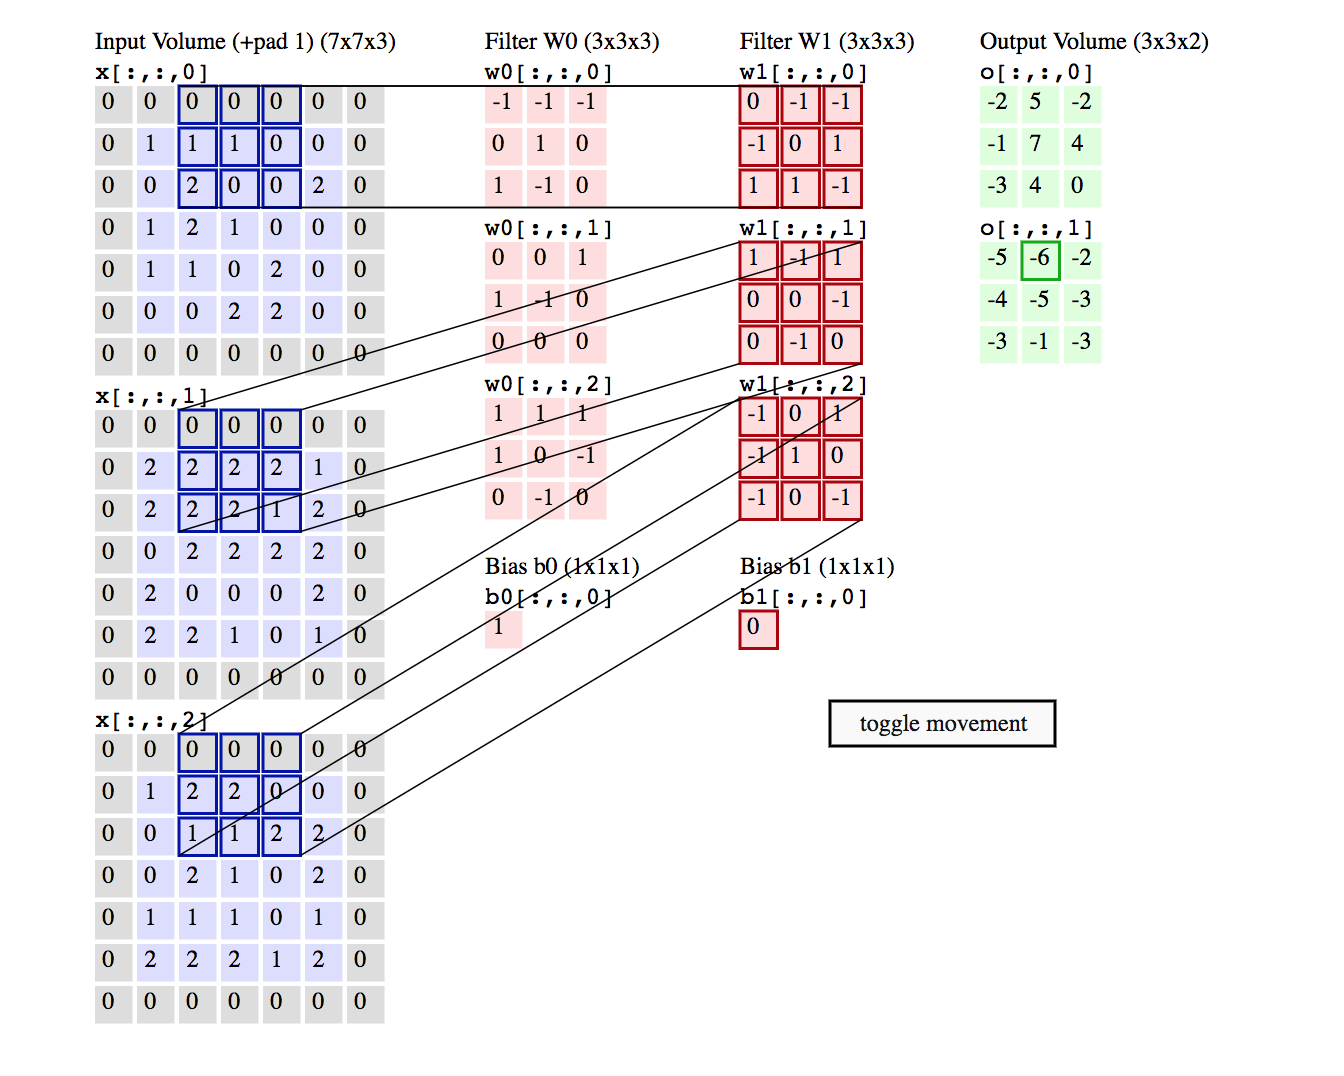
\includegraphics[width=135mm,height=100mm]{cnnstructure.png}\cite{cnnpic}
After getting the images we need, I center the image by substract mean and divide it by its standard deviation. Then, I implement the neural networks. The implementation uses Google neural networks' libarary tensorflow. First, we have 5 convolutional layers. For each layer, we take the previous layer as the input. Then, we specify some kernel size,(for this lab, I specify as (4,4)) some filter numbers,(it can be varied and gives us different models) and some stride(I set it to be 2 for every layer) with paddings if necessary by calling $tensorflow$ library function.  $tf.contrib.layers.conv2d$\cite{conv2d} For the specific parameters, I will discuss in the result part. Then I have a fully connected layer with output of $num_output=10$ as we have 10 different classes of possible input. An visualization of fully connected layer can be seen as below
\par
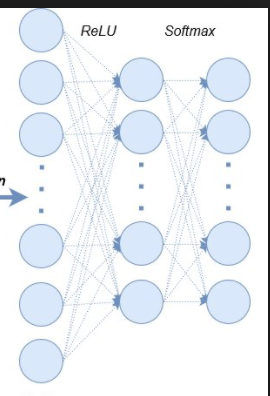
\includegraphics[width=135mm,height=100mm]{full.png}\cite{full}
\subsection{Optimization}
After getting the output tensor, we compute the softmax cross entropy difference between the actual value ($label$) and the output value we get ($convolution$ $network$). In order to do this, we call $tf.nn.sparsesoftmaxcrossentropywithlogits$\cite{logit}.
Later, we set learning rate and the vector parameters to reduce random errors by using momentum optimizer by setting the learning rate to be 0.0001 and momentum to be 0.9. 
\subsection{Training Data}
I train the model for 20 iterations. For each time, it randomly shuffles the pictures we have and take out 32 of them for training. The latter iteration is built on the previous one.
\subsection{Testing Model}
After train the model, I put in all the $10000$ images with label testing data for testing to see how the accuracy is.
\section{Result}
	Let us examine effects of differences on $numoutputs$ can have on our accuracy. The $numoutputs$ reflect how many filters I have. In order to do so, we need to keep other parameters unchanged. To be specific, I set $kernelsize = [4,4]$, which means I only operates on $4x4$ kernel once at a time. stride = 2, it means every time we jump 2 pixels to the next. $padding= same$, which is same to what described in the big picture described above. In this case, we set it to be $0$ to expand pictures so that I can operates on the border case. I consider three different models, monotone increasing outputs, monotone decreasing outputs and decrease first then increase. They give us different result as shown below.
	
	\par
	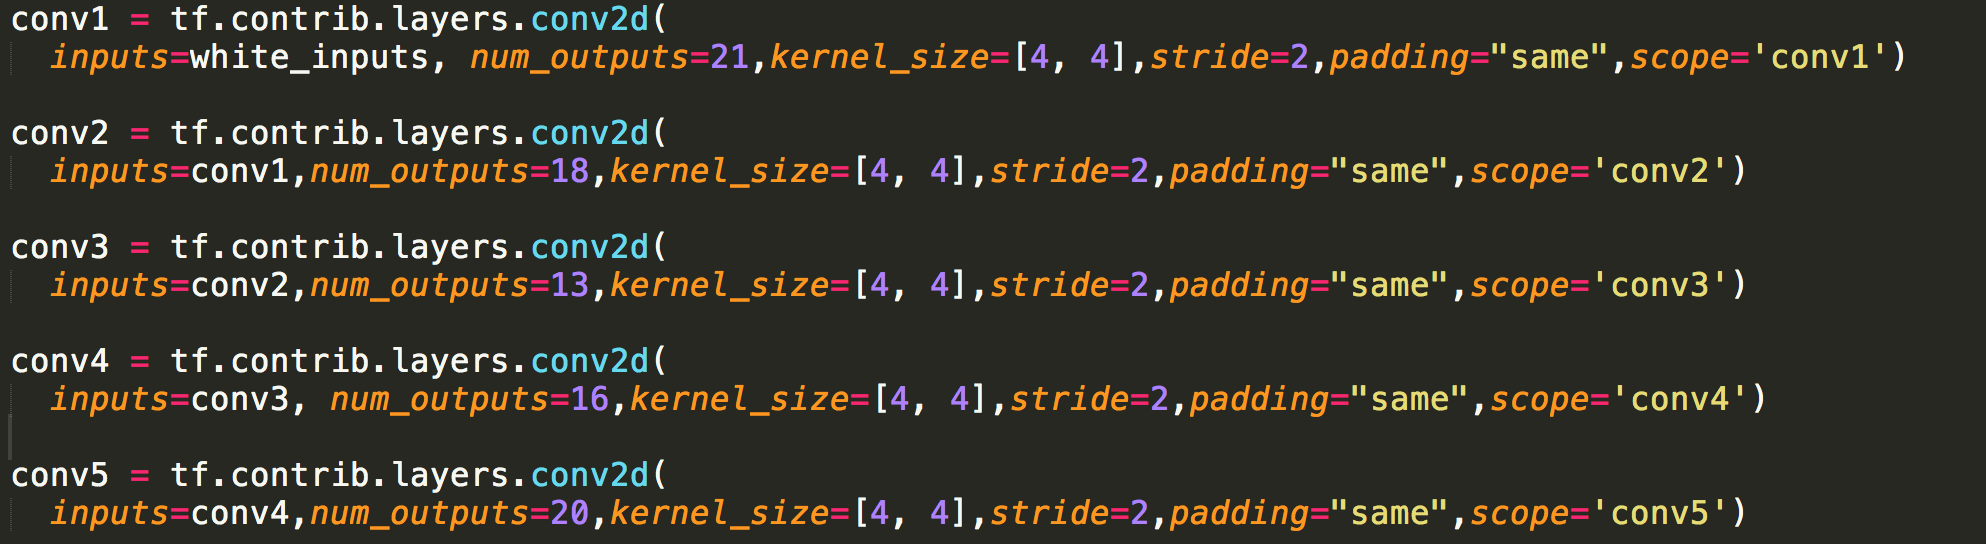
\includegraphics[width=135mm,height=80mm]{model1.png}
	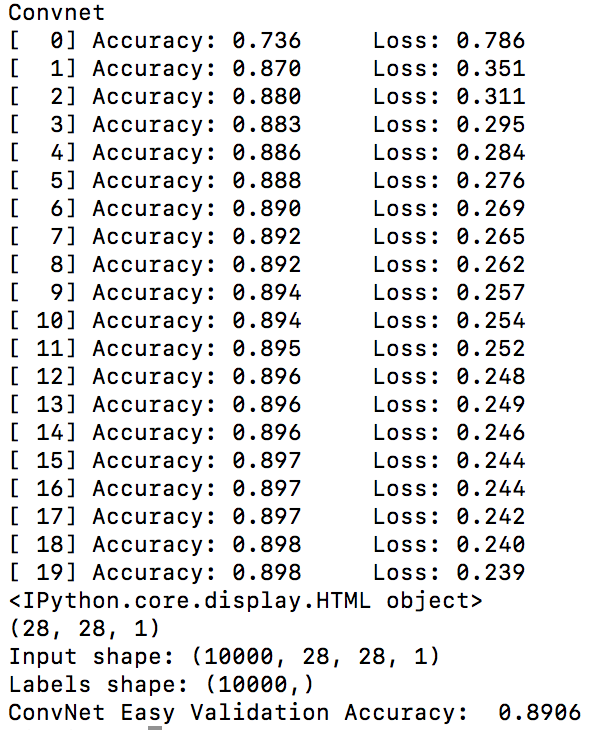
\includegraphics[width=135mm,height=80mm]{result1.png}
	\par For monotone part, the network setup is similar to the screen shot given above. The monotone decreasing part, I set numoutputs for each layer to be 21,18,15,12,9 respectively.
	\par
		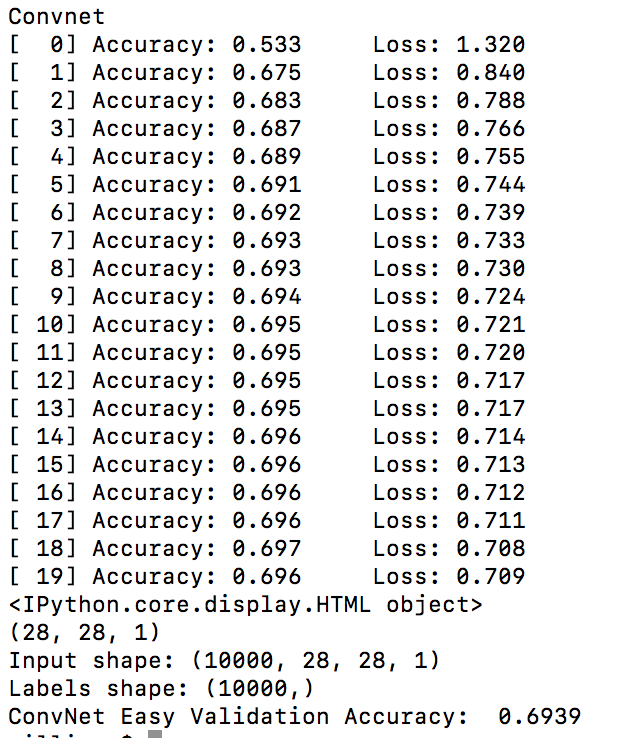
\includegraphics[width=135mm,height=100mm]{result2.png}
	 the monotone increasing part, I reverse them and make it 9,12,15,18,21.
	 The performance is shown below:
	 \par
	 	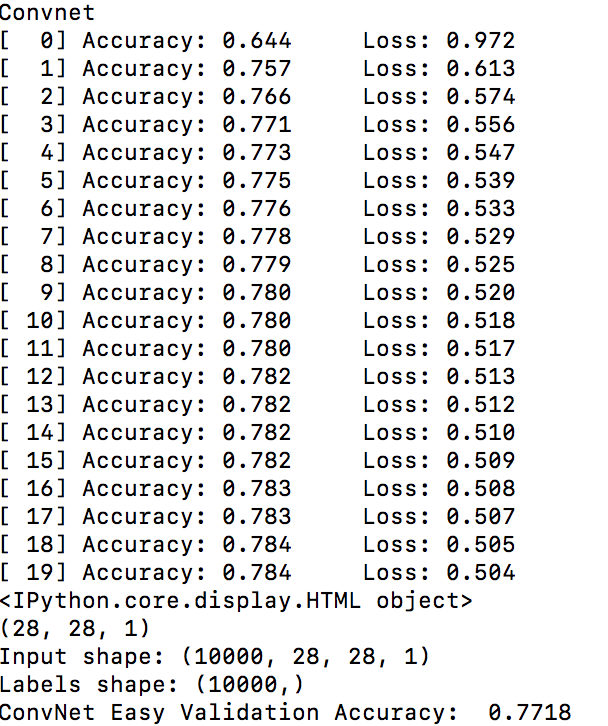
\includegraphics[width=135mm,height=80mm]{increase.png}
	 
	
\section{Conclusion}
As our goal is to classify the digit, the higher the accuracy, the better the model. With the result shown above,  we can get a preliminary conclusion that the number of output with decreasing first and then increasing works best while the monotone increasing works second and monotone decreasing one works the worst. This only is a preliminary result. Many different factors still need to take into consideration. As every iteration we pick different images from the traning set randomly, it is possible that the model stuck in a small interval given its small learning rate. Also, these handwritting pictures may not the most representable one and the testing picture may contain some new feature that the training image does not has. Even the test image gives us high accuracy, we still can't guarantee it works best as the typicalness of those pictures are highly susceptible.
\begin{thebibliography}{9}
	\bibitem{full}
	Andy 
	\textit{Convolutional Neural Networks Tutorial in TensorFlow}
	\textit{http://adventuresinmachinelearning.com/convolutional-neural-networks-tutorial-tensorflow/}
	\bibitem{cnnpic}
	Justin Johnson
	\textit{Convolutional Neural Networks (CNNs / ConvNets)}
	\textit{http://cs231n.github.io/convolutional-networks/}
	\bibitem{code}
	Philipp Krähenbühl
	\textit{CS 342 - Homework 4}
	\textit{http://www.philkr.net/cs342/homework/04/}
	
	
	\bibitem{conv2d} 
	Tensorflow. 
	\textit{tf.contrib.layers.conv2d}. [\textit{https://www.tensorflow.org/apidocs/python/tf/contrib/layers/conv2d}]. 
	, 2017.
		\bibitem{logit} 
	Tensorflow. 
	\textit{$tf.nn.sparse_softmax_cross_entropy_with_logits$}. [\textit{$https://www.tensorflow.org/api_docs/python/tf/nn/sparse_softmax_cross_entropy_with_logits$}]. 
	, 2017.
	
	
	
\end{thebibliography}
\end{document}